\section{Pair breaking by dark matter}\label{sec:15.1}

A dark-matter particle of \SI{1}{keV} that scatters in aluminum deposits at most \SI{3.5}{meV}, about ten times the pair-breaking threshold, and transfers at most \SI{5.3}{eV} of momentum. To deposit $\omega$ it must transfer at least $q = \omega/v_{\mathrm{max}}$, with $v_{\mathrm{max}} = 2.650\times10^{-3}$ the largest speed of a halo particle in the laboratory (\cref{eq:1.2-vmax}). The line $q = \omega/v_{\mathrm{max}}$ in the $(q,\omega)$ plane, the \emph{kinematic edge}, is a different object from the \emph{pair-breaking edge} $\omega = 2\Delta_{\mathrm{BCS}}$, the threshold in energy. The ratio of the gap to the Doppler width of the Fermi surface is $\Delta_{\mathrm{BCS}}/qv_{\mathrm{F}} = (v_{\mathrm{max}}/v_{\mathrm{F}})(\Delta_{\mathrm{BCS}}/\omega)$, and it takes its largest value on the kinematic edge, 0.20 at the threshold. \Cref{sec:7.2} found that this ratio controls the correction that restores charge conservation. We build the loss function from the conserving response of \cref{eq:7.2-Rc}. Two truncations of the conserving response are accurate far above the pair-breaking edge: the Lindhard function of the normal metal, and the same function multiplied by the case-I coherence factor of \cref{eq:7.2-pairspec}.

\subsection{The loss-function rate of a superconductor}\label{sec:15.1-rate}

A mediator that couples to the electron number acts through the density row of the master formula, with $\mathfrak{D}_{ee} = |\tilde V(\vect{q})|^2$ and $S = (2q^2/e^2)\,L/(1 - \ee^{-\beta\omega})$ (\cref{sec:10.2}). At \SI{10}{mK} the threshold has $\beta\omega = 418$, so the thermal factor is one, and the spectrum is \cref{eq:10.2-rate} with $\bar L$ replaced by the loss function of the superconductor, which is isotropic in the model used here. For a dark photon, which couples to the total charge, this spectrum is exact. For a mediator that couples to electrons alone it holds with the nuclei clamped, and the lattice then enters only through the pairing interaction already contained in $\Delta_{\mathrm{BCS}}$. The ions' own response appears in the loss function through the phonon pole at $\omega = c_{\mathrm{LA}}q$, and above that pole the ionic response is a correction of relative order $(c_{\mathrm{LA}}q/\omega)^2$. The longitudinal sound speed along [100] is $c_{\mathrm{LA}} = (C_{11}/\rho)^{1/2} = \SI{6.47}{km.s^{-1}}$, from the zero-temperature elastic constant $C_{11} = \SI{114.3}{GPa}$~\cite[Table~2]{malica2020quasi} and the low-temperature density $\rho = \SI{2.73}{g.cm^{-3}}$. The correction is then $(c_{\mathrm{LA}}/v_{\mathrm{max}})^2 = \num{6.6e-5}$ on the kinematic edge. For $\mchi < \SI{3.2}{keV}$ even the largest momentum transfer, $2\mchi v_{\mathrm{max}}$, excites phonons only below $2\Delta_{\mathrm{BCS}}$.

The dielectric function is the proper density response screened by the Coulomb interaction, $\varepsilon = 1 - v_{\mathrm{C}}(q)\tilde R$ (\cref{sec:4.4}). In the normal metal the random-phase approximation puts the independent-particle bubble in place of $\tilde R$, and the result is the Lindhard function of \cref{eq:4.5-rpa}. In the superconductor, however, the proper response must itself conserve charge, and \cref{sec:7.2} showed that the bare quasiparticle bubble does not. The conserving response is the time-dependent mean field in the three Nambu channels $(\boldsymbol{\eta}, \mathsf{s}_1, \mathsf{s}_2)$ of \cref{eq:7.2-nambu}, the pair-field ladder of \cref{eq:7.2-Rc}~\cite{anderson1958random}. In field-theory language the ladder is the vertex correction that restores the Ward identity of charge. Adding the Coulomb interaction in the density channel gives the generalized random-phase approximation:
\begin{keyresult}[Conserving loss function of a superconductor]
\begin{equation}
  \varepsilon^{\mathrm{cons}}(q,\omega) = 1 - v_{\mathrm{C}}(q)\,R^{\mathrm{cons}}(q,\omega), \qquad
  L^{\mathrm{cons}}(q,\omega) = \Imag\Bigl[-\frac{1}{\varepsilon^{\mathrm{cons}}(q,\omega)}\Bigr] ,
  \label{eq:15.1-Lcons}
\end{equation}
with $R^{\mathrm{cons}} = R_{\boldsymbol{\eta}\boldsymbol{\eta}}$ the density response of \cref{eq:7.2-Rc}, which contains the pair-field ladder and no Coulomb interaction.
\end{keyresult}
\noindent The Coulomb interaction is a function of the local density and commutes with it, so the screened response obeys the continuity equation and the f-sum rule whenever $R^{\mathrm{cons}}$ does (\cref{sec:7.2}). The core electrons of aluminum add a constant of order one to $\varepsilon$, negligible against $k_{\mathrm{TF}}^2/q^2 \ge \num{5.8e5}$ for $q \le \SI{5.3}{eV}$. Here $k_{\mathrm{TF}} = \SI{4.05}{keV}$ is the Thomas--Fermi wavevector of the free-electron gas of aluminum: three electrons per atom in the fcc cell of side $a = \SI{4.05}{\angstrom}$, so $\nd_e = \SI{1.81e23}{cm^{-3}}$, $k_{\mathrm{F}} = \SI{1.75}{\angstrom^{-1}}$, the bare electron mass, $v_{\mathrm{F}} = k_{\mathrm{F}}/m_e = \num{6.75e-3}$ and $\omega_p = \SI{15.78}{eV}$. The amplitude channel $\mathsf{s}_1$ decouples from the density in a metal whose density of states is symmetric about the Fermi level (\cref{sec:7.2}); the asymmetry over the energy range of the pairs is of relative order $\Delta_{\mathrm{BCS}}/E_{\mathrm{F}} = \num{1.5e-5}$, and we drop it.

\subsection{The conserving response in closed form}\label{sec:15.1-closed}

For aluminum we set the temperature to zero, take the density of states $\mathcal{N}_{\mathrm{F}}$ constant over the energies of the pairs, and take the metal clean. We also linearize the band across the shell, $\xi_{\vect{k}+\vect{q}} = \xi_{\vect{k}} + v_{\mathrm{F}}q\mu$ with $\mu$ the cosine of the angle between $\vect{k}$ and $\vect{q}$. The dropped term $q^2/2m_e$ is below \SI{3e-5}{eV} for $q \le \SI{5.3}{eV}$, whereas $v_{\mathrm{F}}q \ge 2.5\,\omega$. With these simplifications every bubble of \cref{eq:7.2-Rc} reduces to one function. At $T = 0$ the density and pair operators either create a pair of quasiparticles, with energy $E + E'$ for $E = E_{\vect{k}}$ and $E' = E_{\vect{k}+\vect{q}}$, or destroy one, and the bubbles are
\begin{equation}
  R^0_{AB}(q,\omega) = \frac{1}{\Vol}\sum_{\vect{k}}\Bigl[\frac{M^{\mathrm{N}*}_AM^{\mathrm{N}}_B}{\omega - E - E' + \ii0^+} - \frac{M^{\mathrm{N}}_AM^{\mathrm{N}*}_B}{\omega + E + E' + \ii0^+}\Bigr] ,
  \label{eq:15.1-bubble}
\end{equation}
with $M^{\mathrm{N}}_A$ the amplitude with which the Nambu-channel operator $O_A$ (superscript N for Nambu) creates the pair. For the density it is $M^{\mathrm{N}}_{\boldsymbol{\eta}} = uv' + vu'$ of \cref{eq:7.2-coh}. The phase operator is $O_{\mathsf{s}_2} = -\ii(B^\dagger_{\vect{q}} - B_{-\vect{q}})$, with $B^\dagger_{\vect{q}}$ the pair creation operator of \cref{app:D.21}. It therefore creates the same pair through $B^\dagger_{\vect{q}}$, with the amplitude $M^{\mathrm{N}}_{\mathsf{s}_2} = -\ii(uu' + vv')$; this phase reproduces $R^0_{\mathsf{s}_2\boldsymbol{\eta}}$ of \cref{sec:7.2} at $q = 0$, and the sign of the ladder below does not depend on it. With \cref{eq:7.2-E},
\begin{gather*}
  |M^{\mathrm{N}}_{\boldsymbol{\eta}}|^2 = \frac{EE' - \xi\xi' + \Delta_{\mathrm{BCS}}^2}{2EE'}, \qquad
  |M^{\mathrm{N}}_{\mathsf{s}_2}|^2 = \frac{EE' + \xi\xi' + \Delta_{\mathrm{BCS}}^2}{2EE'}, \\
  M^{\mathrm{N}*}_{\boldsymbol{\eta}}M^{\mathrm{N}}_{\mathsf{s}_2} = -\frac{\ii\Delta_{\mathrm{BCS}}(E + E')}{2EE'} ,
\end{gather*}
where the mixed product follows from $(uv' + vu')(uu' + vv') = u'v'(u^2 + v^2) + uv(u'^2 + v'^2) = \Delta_{\mathrm{BCS}}/2E' + \Delta_{\mathrm{BCS}}/2E$.

The linear band turns these three products into functions of $E + E'$. Since $E^2 = \xi^2 + \Delta_{\mathrm{BCS}}^2$, the product $(EE' + \xi\xi' + \Delta_{\mathrm{BCS}}^2)(EE' - \xi\xi' - \Delta_{\mathrm{BCS}}^2) = E^2E'^2 - (\xi\xi' + \Delta_{\mathrm{BCS}}^2)^2$ equals $\Delta_{\mathrm{BCS}}^2(\xi' - \xi)^2$, and $EE' + \xi\xi' + \Delta_{\mathrm{BCS}}^2$ is half of $(E + E')^2 - (\xi' - \xi)^2$. For the density amplitude we write $EE' - \xi\xi' + \Delta_{\mathrm{BCS}}^2 = (EE' - \xi\xi' - \Delta_{\mathrm{BCS}}^2) + 2\Delta_{\mathrm{BCS}}^2$ and use the product for the first bracket. With $\xi' - \xi = v_{\mathrm{F}}q\mu$,
\begin{equation}
  EE' + \xi\xi' + \Delta_{\mathrm{BCS}}^2 = \tfrac12\bigl[(E + E')^2 - v_{\mathrm{F}}^2q^2\mu^2\bigr], \qquad
  |M^{\mathrm{N}}_{\boldsymbol{\eta}}|^2 = \frac{\Delta_{\mathrm{BCS}}^2(E + E')^2}{EE'\bigl[(E + E')^2 - v_{\mathrm{F}}^2q^2\mu^2\bigr]} .
  \label{eq:15.1-ident}
\end{equation}
The quantity $\omega_\mu^2 = \omega^2 - v_{\mathrm{F}}^2q^2\mu^2$ is the energy of the pair in the frame that moves with the Doppler shift, and a pair at angle $\mu$ can be created only if $\omega_\mu \ge 2\Delta_{\mathrm{BCS}}$, the counterpart of the threshold \cref{eq:7.2-threshold}. The remaining integral is the $q = 0$ pair sum $F(\omega)$ of \cref{sec:7.2}, now at each angle. A hyperbolic substitution evaluates it (\cref{app:D.39}):
\begin{equation}
  F_\mu(\omega) = \frac{\mathcal{N}_{\mathrm{F}}}{2}\int\dd\xi\,\frac{E + E'}{EE'\,\bigl[\omega^2 - (E + E')^2\bigr]}
  = -\frac{\mathcal{N}_{\mathrm{F}}}{2\Delta_{\mathrm{BCS}}^2}\,\frac{\arcsin\sqrt{\mathfrak{p}_\mu}}{\sqrt{\mathfrak{p}_\mu(1 - \mathfrak{p}_\mu)}}, \qquad
  \mathfrak{p}_\mu = \frac{\omega_\mu^2}{4\Delta_{\mathrm{BCS}}^2} ,
  \label{eq:15.1-F}
\end{equation}
for $0 < \mathfrak{p}_\mu < 1$, with $F_0 = F$, and continued to the other ranges of $\mathfrak{p}_\mu$ in \cref{eq:D.39-Fcont}. Only at $\mathfrak{p}_\mu > 1$, where pairs can be created, is $F_\mu$ complex.

The density bubble follows from \cref{eq:15.1-bubble,eq:15.1-ident} with $\Vol^{-1}\sum_{\vect{k}} \to \mathcal{N}_{\mathrm{F}}\int\dd\xi\int_{-1}^1\dd\mu/2$. Splitting the integrand of the density bubble by partial fractions into an $F_\mu$ term and an elementary term, and using the gap equation, gives (\cref{app:D.39}), with $\langle X\rangle_\mu = \int_0^1\dd\mu\,X$,
\begin{equation}
  \begin{gathered}
  R^0_{\boldsymbol{\eta}\boldsymbol{\eta}} = \Bigl\langle\frac{2\mathcal{N}_{\mathrm{F}}v_{\mathrm{F}}^2q^2\mu^2 + 4\Delta_{\mathrm{BCS}}^2\omega^2F_\mu}{\omega_\mu^2}\Bigr\rangle_\mu, \\
  R^0_{\mathsf{s}_2\boldsymbol{\eta}} = -R^0_{\boldsymbol{\eta}\mathsf{s}_2} = 2\ii\Delta_{\mathrm{BCS}}\,\omega\,\langle F_\mu\rangle_\mu, \qquad
  1 + \tfrac12V_{\mathrm{BCS}}R^0_{\mathsf{s}_2\mathsf{s}_2} = \tfrac12V_{\mathrm{BCS}}\langle\omega_\mu^2F_\mu\rangle_\mu .
  \end{gathered}
  \label{eq:15.1-bubbles}
\end{equation}
At $q = 0$ these three expressions are the bubbles of \cref{sec:7.2}. The last expression is the denominator of the phase channel in \cref{eq:7.2-Rc}, and the coupling $V_{\mathrm{BCS}}$ drops out of the result:
\begin{keyresult}[Conserving density response of a clean superconductor]
\begin{equation}
  R^{\mathrm{cons}}(q,\omega) = \underbrace{\Bigl\langle\frac{2\mathcal{N}_{\mathrm{F}}v_{\mathrm{F}}^2q^2\mu^2 + 4\Delta_{\mathrm{BCS}}^2\omega^2F_\mu(\omega)}{\omega^2 - v_{\mathrm{F}}^2q^2\mu^2}\Bigr\rangle_\mu}_{\text{bare bubble } R^0_{\boldsymbol{\eta}\boldsymbol{\eta}}}
  \;\underbrace{-\;\frac{4\Delta_{\mathrm{BCS}}^2\omega^2\,\langle F_\mu(\omega)\rangle_\mu^2}{\langle(\omega^2 - v_{\mathrm{F}}^2q^2\mu^2)F_\mu(\omega)\rangle_\mu}}_{\text{pair-field ladder}} ,
  \label{eq:15.1-Rcons}
\end{equation}
with $F_\mu$ of \cref{eq:15.1-F}, for $T = 0$, constant $\mathcal{N}_{\mathrm{F}}$, a linear band and no impurities.
\end{keyresult}
\noindent At $q = 0$ the ladder cancels the bubble for every $\omega$, as \cref{eq:7.2-cancel} states. At small $q$ the cancellation is incomplete, and $R^{\mathrm{cons}} \to 2\mathcal{N}_{\mathrm{F}}v_{\mathrm{F}}^2q^2/3\omega^2 = \nd_eq^2/m_e\omega^2$, the free-particle tail whose coefficient is the f-sum rule; at $v_{\mathrm{F}}q = 0.01\,\Delta_{\mathrm{BCS}}$, $R^{\mathrm{cons}}$ and the free-particle tail agree to one part in $10^5$, while the bare bubble stays at its $q = 0$ value. At $\omega \to 0$ the bubble gives $-2\mathcal{N}_{\mathrm{F}}$, the Thomas--Fermi value, and the ladder vanishes: pairing leaves the static screening of the metal unchanged. As $\Delta_{\mathrm{BCS}} \to 0$ at fixed $\omega/qv_{\mathrm{F}}$, the conserving response approaches the Lindhard function at $q \ll k_{\mathrm{F}}$, to \num{6e-5} at $v_{\mathrm{F}}q = 10^3\,\Delta_{\mathrm{BCS}}$ and \num{8e-7} at $10^4\,\Delta_{\mathrm{BCS}}$.

Below $2\Delta_{\mathrm{BCS}}$ no pairs can be created, $F_\mu$ is real, and $L^{\mathrm{cons}}$ vanishes except where $\varepsilon^{\mathrm{cons}}$ does. The denominator of the ladder vanishes at one frequency $\varOmega_{\mathrm{AB}}(q) < 2\Delta_{\mathrm{BCS}}$: the Anderson--Bogoliubov mode of \cref{sec:7.2}, the Goldstone mode of the broken phase symmetry, now at finite $q$. There $R^{\mathrm{cons}}$ has a pole, so $\varepsilon^{\mathrm{cons}}$ has one too and the loss function has a zero, not a peak. The Coulomb interaction moves the weight of the mode to the plasmon, as \cref{sec:7.2} anticipated (the Anderson--Higgs mechanism), and a sum rule proves that no loss weight is left below $2\Delta_{\mathrm{BCS}}$ (\cref{app:D.39}). Through the Kramers--Kronig relation the pole still shifts $\Real\varepsilon^{\mathrm{cons}}$ above $2\Delta_{\mathrm{BCS}}$. On the kinematic edge at $\omega = 2.2\,\Delta_{\mathrm{BCS}}$, the pole term alone exceeds the whole shift of $\Real\varepsilon^{\mathrm{cons}}$ relative to the Lindhard function, and there the rest of the ladder acts the other way. The pole term is \SI{58}{\percent} of the shift at $2.5\,\Delta_{\mathrm{BCS}}$, \SI{16}{\percent} at $3\Delta_{\mathrm{BCS}}$, and zero at $5\Delta_{\mathrm{BCS}}$, where the edge momentum has pushed the mode into the pair continuum. The pole explains the shift only for $y \lesssim 2.3$.

The clean limit needs only $\mathcal{N}_{\mathrm{F}}$, $v_{\mathrm{F}}$ and $\Delta_{\mathrm{BCS}}$, and no first-principles calculation.

\subsection{The case-I coherence factor}\label{sec:15.1-bare}

Without the ladder the density response is the bare bubble $R^0_{\boldsymbol{\eta}\boldsymbol{\eta}}$, with the dielectric function $\varepsilon^{\mathrm{bare}} = 1 - v_{\mathrm{C}}R^0_{\boldsymbol{\eta}\boldsymbol{\eta}}$. The absorptive part of $\varepsilon^{\mathrm{bare}}$ comes from the imaginary part of $F_\mu$ alone, $\Imag F_\mu = -\pi\mathcal{N}_{\mathrm{F}}/[4\Delta_{\mathrm{BCS}}^2\sqrt{\mathfrak{p}_\mu(\mathfrak{p}_\mu - 1)}]$ for $\omega_\mu > 2\Delta_{\mathrm{BCS}}$. Changing the variable of the angular average from $\mu$ to $\omega_\mu$, $\dd\mu = -\omega_\mu\,\dd\omega_\mu/[v_{\mathrm{F}}q(\omega^2 - \omega_\mu^2)^{1/2}]$, gives
\begin{equation*}
  \Imag R^0_{\boldsymbol{\eta}\boldsymbol{\eta}} = -\frac{4\pi\mathcal{N}_{\mathrm{F}}\Delta_{\mathrm{BCS}}^2\omega^2}{v_{\mathrm{F}}q}\int_{2\Delta_{\mathrm{BCS}}}^{\omega}\frac{\dd\omega'}{\omega'^2\sqrt{\omega'^2 - 4\Delta_{\mathrm{BCS}}^2}\,\sqrt{\omega^2 - \omega'^2}} ,
\end{equation*}
provided $v_{\mathrm{F}}q \ge (\omega^2 - 4\Delta_{\mathrm{BCS}}^2)^{1/2}$, so that the whole interval of $\omega_\mu$ lies inside $0 \le \mu \le 1$. The normal metal has $\Imag R^0 = -\pi\mathcal{N}_{\mathrm{F}}\omega/v_{\mathrm{F}}q$ below $\omega = qv_{\mathrm{F}}$ (\cref{sec:4.5}). The ratio of the superconducting to the normal absorptive part depends on $y = \omega/\Delta_{\mathrm{BCS}}$ alone:
\begin{keyresult}[Absorptive part of the bare quasiparticle bubble]
\begin{equation}
  \begin{gathered}
  \Imag\varepsilon^{\mathrm{bare}}(q,\omega) = \mathfrak{g}_{\mathrm{I}}\Bigl(\frac{\omega}{\Delta_{\mathrm{BCS}}}\Bigr)\,\Imag\varepsilon_{\mathrm{Lin}}(q,\omega) \qquad \bigl(v_{\mathrm{F}}q \ge (\omega^2 - 4\Delta_{\mathrm{BCS}}^2)^{1/2}\bigr), \\
  \mathfrak{g}_{\mathrm{I}}(y) = 4y\int_2^y\frac{\dd u}{u^2\sqrt{u^2 - 4}\sqrt{y^2 - u^2}} = \Bigl(1 + \frac{2}{y}\Bigr)\mathrm{E}(k) - \frac{4\,\mathrm{K}(k)}{y + 2}, \qquad k = \frac{y - 2}{y + 2} ,
  \end{gathered}
  \label{eq:15.1-gI}
\end{equation}
with $\mathrm{K}$ and $\mathrm{E}$ the complete elliptic integrals of the first and second kind of modulus $k$, for $y > 2$; $\mathfrak{g}_{\mathrm{I}} = 0$ below.
\end{keyresult}
\noindent The function $\mathfrak{g}_{\mathrm{I}}$ is the case-I ratio $S_{\mathrm{I}}/S_{\mathrm{n}}$ of \cref{eq:7.2-pairspec}, obtained there by counting pairs in the energies of the two quasiparticles and here by integrating over the angle; the two integrals agree with the elliptic form to $10^{-12}$. It jumps to $\pi/2$ at $y = 2$, is 1.322 at $y = 3$ and 1.051 at $y = 10$, and \cref{tab:15-edge} lists it at the other energies we use. Allen's theory of phonon-assisted absorption in metals contains the elliptic form~\cite{allen1971electron}, as quoted by Hochberg, Lin and Zurek~\cite[Eq.~(17)]{hochberg2016absorption}. The corresponding case-II form is that of Mattis and Bardeen~\cite{mattis1958theory}. Under the simplifications above, \cref{eq:15.1-gI} is exact: the absorptive part of the bare bubble carries no correction in powers of $\Delta_{\mathrm{BCS}}/qv_{\mathrm{F}}$. The validity condition of \cref{eq:15.1-gI} holds for every momentum transfer of halo dark matter, since $v_{\mathrm{F}}q \ge v_{\mathrm{F}}\omega/v_{\mathrm{max}} = 2.5\,\omega$.

The pair-field ladder changes the absorptive part. Its relative size is the vertex fraction $\mathfrak{v} = \Imag(R^{\mathrm{cons}} - R^0_{\boldsymbol{\eta}\boldsymbol{\eta}})/\Imag R^0_{\boldsymbol{\eta}\boldsymbol{\eta}}$, which follows from \cref{eq:15.1-Rcons} by quadrature over $\mu$ (\cref{app:D.39}). On the kinematic edge the vertex fraction is largest near the threshold, $+0.44$ at $y = 2.2$, and falls to $+0.004$ at $y = 10$ (\cref{tab:15-edge}). The vertex fraction does not fall monotonically with $q$, however: at $y = 5$ it is $+0.052$ on the edge and still $+0.044$ at four times the edge momentum, and at $y = 10$ it is nearly three times larger at that momentum than on the edge.

At the threshold itself the ladder replaces the jump of \cref{eq:7.2-pairspec} by a steep rise. The bare absorptive part jumps to $\pi/2$ times the normal value at $y = 2$; in the conserving response it starts from zero and rises steeply. At the edge momentum of $y = 2.05$, $\Imag\varepsilon^{\mathrm{cons}}/\Imag\varepsilon_{\mathrm{Lin}}$ is 0.14 at $y - 2 = 10^{-6}$, 0.64 at $10^{-3}$ and 1.30 at $10^{-2}$, and it passes the bare value $\pi/2$ before $y - 2 = 0.03$, that is within \SI{5}{\micro eV} of the threshold. For a rate integrated over energy, the conserving response therefore keeps a step at $2\Delta_{\mathrm{BCS}}$, smoothed over a few microelectronvolts. The conserving loss function vanishes at $2\Delta_{\mathrm{BCS}}$ with its absorptive part and is back to $0.97\,L^{\mathrm{nor}}$ by $y - 2 = 0.03$, with $L^{\mathrm{nor}} = \Imag[-1/\varepsilon_{\mathrm{Lin}}]$.

\begin{figure}[tbp]
  \centering
  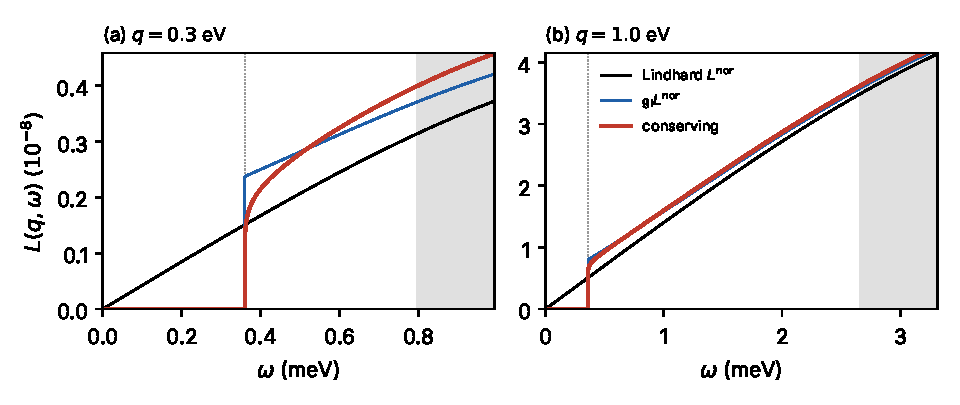
\includegraphics[width=\linewidth]{figures/ch15/fig15_1.pdf}
  \caption{Loss function of aluminum near the pair-breaking edge at the momentum transfers (a) $q = \SI{0.3}{eV}$ and (b) $q = \SI{1}{eV}$, against the energy $\omega$, for the bulk gap $\Delta_{\mathrm{BCS}} = \SI{0.18}{meV}$ (dotted line at $2\Delta_{\mathrm{BCS}}$). Red: conserving response, \cref{eq:15.1-Lcons,eq:15.1-Rcons}; blue: the case-I factor times the normal loss function, $\mathfrak{g}_{\mathrm{I}}L^{\mathrm{nor}}$; black: Lindhard loss function of the normal metal, $L^{\mathrm{nor}}$. Halo dark matter reaches the energies left of the gray band, $\omega \le qv_{\mathrm{max}}$. All curves are clean, $T = 0$, with a constant density of states, $v_{\mathrm{F}} = \num{6.75e-3}$ and $k_{\mathrm{TF}} = \SI{4.05}{keV}$. At \SI{0.3}{eV} and $\omega \ge 2.2\,\Delta_{\mathrm{BCS}}$ the conserving loss function lies 27 to \SI{34}{\percent} above the Lindhard function. At \SI{1}{eV} all three agree within \SI{5}{\percent} at the largest reachable energy.}
  \label{fig:15-alloss}
\end{figure}

At $q = \SI{0.3}{eV}$, $v_{\mathrm{F}}q = 11\,\Delta_{\mathrm{BCS}}$, every energy that halo dark matter can deposit lies within $4.4\,\Delta_{\mathrm{BCS}}$ of zero, and the conserving response lies above the Lindhard function (\cref{fig:15-alloss}). At $q = \SI{1}{eV}$, $v_{\mathrm{F}}q = 38\,\Delta_{\mathrm{BCS}}$, the differences between the three loss functions are confined to the first few $\Delta_{\mathrm{BCS}}$ above the edge.

\subsection{Truncations of the conserving response}\label{sec:15.1-chain}

Keeping the case-I absorptive part \cref{eq:15.1-gI} but screening it with the normal metal gives $\Imag\varepsilon^{\mathrm{bare}}/|\varepsilon_{\mathrm{Lin}}|^2 = \mathfrak{g}_{\mathrm{I}}L^{\mathrm{nor}}$~\cites[Eq.~(10)]{gan2026mean}[Eq.~(2) and text]{hochberg2023directional}. Closing the gap, $\Delta_{\mathrm{BCS}} \to 0$ at fixed $\omega$, leaves the Lindhard loss function~\cite[Eqs.~(1), (S.13)]{hochberg2021determining}, whose unscreened structure factor below $qv_{\mathrm{F}}$ is the free-gas $S_{\mathrm{n}} = m_e^2\omega/\pi q$ of \cref{sec:7.2}~\cite[Eq.~(3.4)]{hochberg2016detecting}. Dropping the ladder and keeping the normal real part are both controlled by $\Delta_{\mathrm{BCS}}/qv_{\mathrm{F}}$. Closing the gap is controlled by $y$ alone, through $\mathfrak{g}_{\mathrm{I}}(y) - 1$. On the kinematic edge both controlling parameters, $\Delta_{\mathrm{BCS}}/qv_{\mathrm{F}}$ and $\mathfrak{g}_{\mathrm{I}}(y) - 1$, are functions of $y$, and each truncation is worst on that edge. Over all momentum transfers that halo dark matter reaches, the clean conserving loss function lies between 0.980 and 1.085 times $\mathfrak{g}_{\mathrm{I}}L^{\mathrm{nor}}$ for $y \ge 3$; \cref{sec:15.2} gives the values on the edge, and \cref{sec:15.3-sc} the change with the mean free path.

\begin{limitbox}[Loss function of a superconductor near the pair-breaking edge][lim:15.1a]
Lindhard loss function $L^{\mathrm{nor}}$ in the rate \cref{eq:10.2-rate}, with $\Imag\varepsilon_{\mathrm{Lin}} = (\pi/2)(k_{\mathrm{TF}}^2/q^2)(\omega/qv_{\mathrm{F}})$ below $qv_{\mathrm{F}}$~\cites[Eqs.~(1), (S.13)]{hochberg2021determining}[Eq.~(3.4)]{hochberg2016detecting}; with the case-I factor, $\mathfrak{g}_{\mathrm{I}}L^{\mathrm{nor}}$~\cites[Eq.~(10)]{gan2026mean}[Eq.~(2) and text]{hochberg2023directional}.
\par\smallskip
{\centering
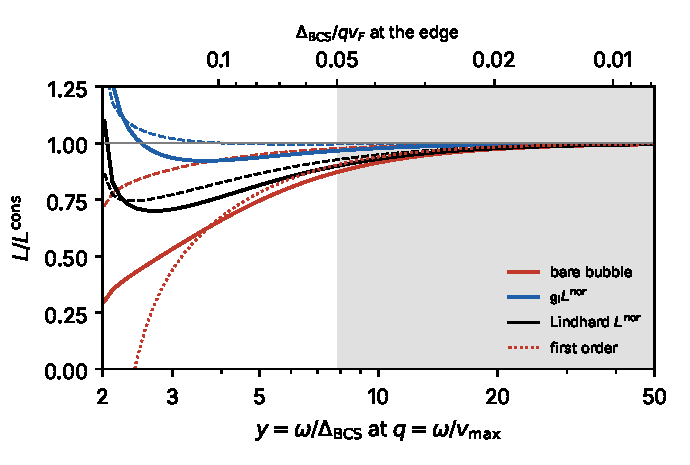
\includegraphics[width=0.92\linewidth]{figures/ch15/limit15_1a.pdf}
\captionof{figure}{Loss function of aluminum on the kinematic edge $q = \omega/v_{\mathrm{max}}$ in two truncations, divided by the conserving loss function \cref{eq:15.1-Lcons}, against $y = \omega/\Delta_{\mathrm{BCS}}$ (top axis: $\Delta_{\mathrm{BCS}}/qv_{\mathrm{F}} = 0.392/y$ there). Blue: $\mathfrak{g}_{\mathrm{I}}L^{\mathrm{nor}}$; black: Lindhard $L^{\mathrm{nor}}$. Dashed: the same at four times the edge momentum. Clean, $T = 0$, constant density of states, $v_{\mathrm{F}} = \num{6.75e-3}$. ``Within \SI{10}{\percent}'' means that the smaller of the two loss functions is at least 0.9 of the larger. Gray: $y \ge 7.9$, where the Lindhard function is within \SI{10}{\percent} of the conserving result on the edge and at all larger momenta. The product $\mathfrak{g}_{\mathrm{I}}L^{\mathrm{nor}}$ is within \SI{10}{\percent} already for $y \ge 2.25$.}\label{fig:15-limit-chain}
\par}
\smallskip
Below $y \approx 3$ on the edge the Lindhard function falls about \SI{30}{\percent} below the conserving loss function, and the clean conserving result itself assumes that impurities do not scatter the electrons within the size of a pair (\cref{sec:15.3-dirty}).
\end{limitbox}

\Cref{fig:15-limit-chain} orders the truncations. The Lindhard function, which has no gap, is within \SI{10}{\percent} of the conserving result for $y \ge 7.9$ on the edge, where $\Delta_{\mathrm{BCS}}/qv_{\mathrm{F}} \le 0.050$, and for $y \ge 6.3$ at four times the edge momentum. At $y = 5$ the Lindhard function is 0.815 of the conserving value on the edge, and the case-I factor $\mathfrak{g}_{\mathrm{I}}(5) = 1.15$ of the conserving response accounts for most of this deficit.

These comparisons are all clean-limit statements. Near the edge the curves are separated by the steep rise of the conserving absorption over a few microelectronvolts, a structure narrower than $\Delta_{\mathrm{BCS}}$. Impurity scattering, at a rate given by $v_{\mathrm{F}}$ over the mean free path, smooths the rise once that rate is no longer small compared with the width of the rise. For $y \ge 3$ the curves depend on functions of $y$ that vary on the scale of $\Delta_{\mathrm{BCS}}$ itself.

\subsection{The aluminum gap and the rate}\label{sec:15.1-al}

The gap enters the loss function through $y = \omega/\Delta_{\mathrm{BCS}}$, in $\mathfrak{g}_{\mathrm{I}}$ and in the ladder, and not only through the threshold. For bulk aluminum it is measured, $\Delta_{\mathrm{BCS}} = \SI{0.18}{meV}$~\cite[Table~III]{savrasov1996electron}, and it agrees within one percent with the weak-coupling value $1.764\,T_c = \SI{0.179}{meV}$ for the measured $T_c = \SI{1.18}{K}$ (\cref{we:7-al}). The value $\Delta = \SI{0.3}{meV}$ often taken for aluminum~\cite[p.~2]{hochberg2023directional} is the film convention $2\Delta_{\mathrm{BCS}} = \SI{0.6}{meV}$ of \cref{sec:1.5}, 1.67 times the bulk value. The film value describes thin films, whose critical temperatures exceed the bulk critical temperature and in ultraclean films approach twice it~\cite{yeh2023doubling}. A rate for a bulk crystal uses \SI{0.18}{meV}. A rate for a film uses the gap measured on that film, and \cref{sec:15.3} adds what the film changes in the response itself.

\begin{workedexample}{The aluminum rate at \SI{1}{keV} with the bulk and the film gap}\label{we:15-alrate}
Take $\mchi = \SI{1}{keV}$, a light mediator, $\FDM = (\alpha m_e/q)^2$, the reference cross section $\sigmae = \SI{e-40}{cm^2}$, the standard halo of \cref{sec:1.2}, and aluminum with $\rho_T = \SI{2.70}{g.cm^{-3}}$, $v_{\mathrm{F}} = \num{6.75e-3}$ and $k_{\mathrm{TF}} = \SI{4.05}{keV}$. The particle deposits at most $\frac12\mchi v_{\mathrm{max}}^2 = \SI{3.51}{meV}$, which is $19.5\,\Delta_{\mathrm{BCS}}$ for the bulk gap and $11.7\,\Delta_{\mathrm{BCS}}$ for the film gap, and transfers at most $2\mchi v_{\mathrm{max}} = \SI{5.30}{eV}$, so that $q/k_{\mathrm{TF}} \le \num{1.3e-3}$ and $v_{\mathrm{F}}q \le 199\,\Delta_{\mathrm{BCS}}$ (bulk). Every point lies in the regime of \cref{eq:15.1-Rcons}.

\Cref{eq:10.2-rate} with the conserving loss function, integrated numerically over $2\Delta_{\mathrm{BCS}} \le \omega \le \SI{3.51}{meV}$ and over the momenta with $\vmin \le v_{\mathrm{max}}$ (Gauss--Legendre sums, in $\omega$ graded toward $2\Delta_{\mathrm{BCS}}$ and in $q$ between the two roots of $\vmin(q,\omega) = v_{\mathrm{max}}$), gives
\begin{equation*}
  \mathcal{R} = \SI{3.26}{kg^{-1}.yr^{-1}}\ (\Delta_{\mathrm{BCS}} = \SI{0.18}{meV}), \qquad
  \mathcal{R} = \SI{2.65}{kg^{-1}.yr^{-1}}\ (\Delta_{\mathrm{BCS}} = \SI{0.30}{meV}) .
\end{equation*}
The bulk gap raises the rate by a factor of 1.23. The lower threshold alone would raise the rate more: with the Lindhard function cut at $2\Delta_{\mathrm{BCS}}$, which has no coherence factor, the factor is 1.30. The difference between the two factors comes from the edge. With the film gap the window $2\Delta_{\mathrm{BCS}} < \omega < 3\Delta_{\mathrm{BCS}}$, where $\mathfrak{g}_{\mathrm{I}}$ is largest, carries \SI{37}{\percent} of the conserving rate; with the bulk gap it carries \SI{20}{\percent}. For a heavy mediator, $\FDM = 1$, the rate at the same cross section is \SI{3.8e-13}{kg^{-1}.yr^{-1}}, and the bulk gap raises it by 1.13.

The choice of loss function matters less than the choice of gap. With the bulk gap and the light mediator, $\mathfrak{g}_{\mathrm{I}}L^{\mathrm{nor}}$ gives 1.010 of the conserving rate, and the Lindhard function cut at the threshold gives 0.850. The normal metal with no gap gives 1.024: at this mass the pile-up of pair states above $2\Delta_{\mathrm{BCS}}$ almost exactly replaces the rate lost below it. With the film gap the same ratios are 1.027, 0.806 and 1.26. These ratios are clean-limit values, and the part of the rate below $3\Delta_{\mathrm{BCS}}$ is the part that impurity scattering can change (\cref{sec:15.3}).
\end{workedexample}
